The fundamental nature of dark matter, which constitutes $\roughly 85\%$ of the matter density and 26\% of the energy density of the Universe, represents a critical gap in our understanding of fundamental physics.
Over the past several decades, experimental searches for particle dark matter have proceeded along several complementary avenues.
Collider experiments (e.g., ATLAS and CMS at the Large Hadron Collider), attempt to produce and detect dark matter particles \citep{Boveia:2018yeb,Ehret:2010mh,Battaglieri:2017aum}.  
Direct detection experiments (e.g., LZ, CDMS, ADMX, PICO, DAMiC, SENSEI, etc.) attempt to directly detect energy deposition from very rare scattering between dark matter and standard model particles \citep{1509:02910, 1804.10697, Du:2018uak}. 
%\AHGP{Cite only US experiments?} 
%\ADW{It was intentional, but perhaps ill advised...}
In parallel, indirect dark matter searches (e.g., {\it Fermi}-LAT, AMS-02, {\it Chandra}, XMM, etc.) seek to detect the energetic Standard Model products from the annihilation or decay of dark matter particles {\it in situ} \citep[\eg][]{1503.02641,1402.2301, 1605.01043, 1603.06978}. 
%\AHGP{Get an axion indirect paper rec from Chanda}
Despite these extensive efforts, the only robust, positive empirical measurement of dark matter continues to come from astrophysical and cosmological observations. 
%\AHGP{This paragraph is fairly WIMP-centric.  I added some axion- and hidden-photon-related refs.}

Astrophysics and cosmology offer a complementary technique to study the fundamental properties of dark matter. 
They probe dark matter directly through gravity, the only force that dark matter is known to couple to, and have established the standard non-relativistic collisionless, cold dark matter (CDM) paradigm.
However, many viable theoretical models of dark matter predict observable deviations from CDM, which are testable with current and future experimental programs.
Fundamental properties of dark matter---e.g., particle mass, self-interaction cross section, coupling to the Standard Model, and time-evolution of dark matter properties---can imprint themselves on the macroscopic distribution of dark matter in a detectable manner.

In addition, astrophysical observations complement particle physics searches by measuring the local distribution of dark matter, targeting indirect searches, and constraining the viable range of dark matter particle mass and electric charge.
As the WIMP paradigm becomes more and more tightly constrained,  astrophysical observations will provide critical information to help direct the evolution of particle physics searches over the coming decade.  
In many cases, observations with telescopes provide \emph{the only} robust, empirical constraints on the viable range of dark matter models.

%\AHGP{I have no idea where these last two sentences are going, especially in light of the next paragraph.  Is the point you're trying to make that knowing the astrophysical distribution of DM can help target astroparticle searches?  Or that these are additional things we can learn with astrophysics?  How much of this paragraph is supposed to focus on constraining the microphysical properties of DM that don't involve standard model interactions, vs. helping sharpen constraints on standard model interactions?}
%\ADW{I've tried to break these into two paragraphs.}

%\ADW{Adapted from Buckley and Peter} 
At the same time, there is immense dark matter discovery potential at the intersection of particle physics and astrophysics.
Detecting a deviation from the gravitational predictions of CDM would provide much-needed experimental guidance on parameters that are not easily measured in particle physics experiments (\eg, dark matter self-interaction cross sections). 
If, on the other hand, all astrophysical studies of dark matter are found to agree with the CDM predictions, the improved knowledge of dark matter distributions will reduce major sources of theoretical uncertainties in the particle physics experiments. 
%ADW: I don't know what is being referred to here.
Likewise, results from particle experiments can either restrict the possible model space relevant to novel astrophysical signals, or suggest specific deviations from the CDM paradigm which can be investigated observationally.

The Large Synoptic Survey Telescope (LSST) is a next-generation wide-area optical survey instrument that will enable high-precision cosmological measurements to probe the fundamental physics of dark matter and dark energy \citep{0805.2366}. Following on predecessors such as the Sloan Digital Sky Survey (SDSS), Pan-STARRS, and the Dark Energy Survey (DES), LSST promises to greatly enhance our knowledge of the dark sector of the Universe. 
LSST will measure the properties of dark matter over a wide range of astrophysical scales. 
At the largest scales, LSST will use gravitational weak lensing and the large scale clustering of galaxies to trace the distribution of dark matter.
At the smallest scales, LSST will trace the distribution of dark matter with the faintest galaxies, gravitational perturbations from dark matter substructure detectable through gravitational strong lensing and tracer stellar populations.
In addition, the temporal component of the LSST ``wide, fast, deep'' survey will open a new window on the search for compact dark matter such as primordial black holes (PBHs).
LSST will provide a rich scientific data set that can be used to develop novel and unanticipated constraints on dark matter properties through precise measurements of physical processes, such as anomalous energy loss in stars that could be produced by axions or axion-like particles.

In this white paper, we present several techniques that LSST will employ to probe the fundamental properties of dark matter. 
Rather than presenting a comprehensive review of astrophysical probes of dark matter  \citep[e.g.,][]{BuckleyPeter:2017} or an extensive discussion of any particular dark matter model \citep[e.g.,][]{Jain:2019}, we choose to focus on what we believe are some of the most exciting opportunities to study dark matter physics with LSST. 
Many astrophysical measurements require collaborative observations between several instruments, and the study of dark matter with LSST is no exception. 
Throughout this paper we describe situations where LSST will complement other astrophysical and particle investigations of dark matter.
Our over-arching goal in this paper is to convince our particle physics colleagues that not only will LSST provide exciting results on the nature of dark matter, but that observations from LSST are {\it essential} for guiding future particle physics searches.

\begin{figure}[t]
\centering
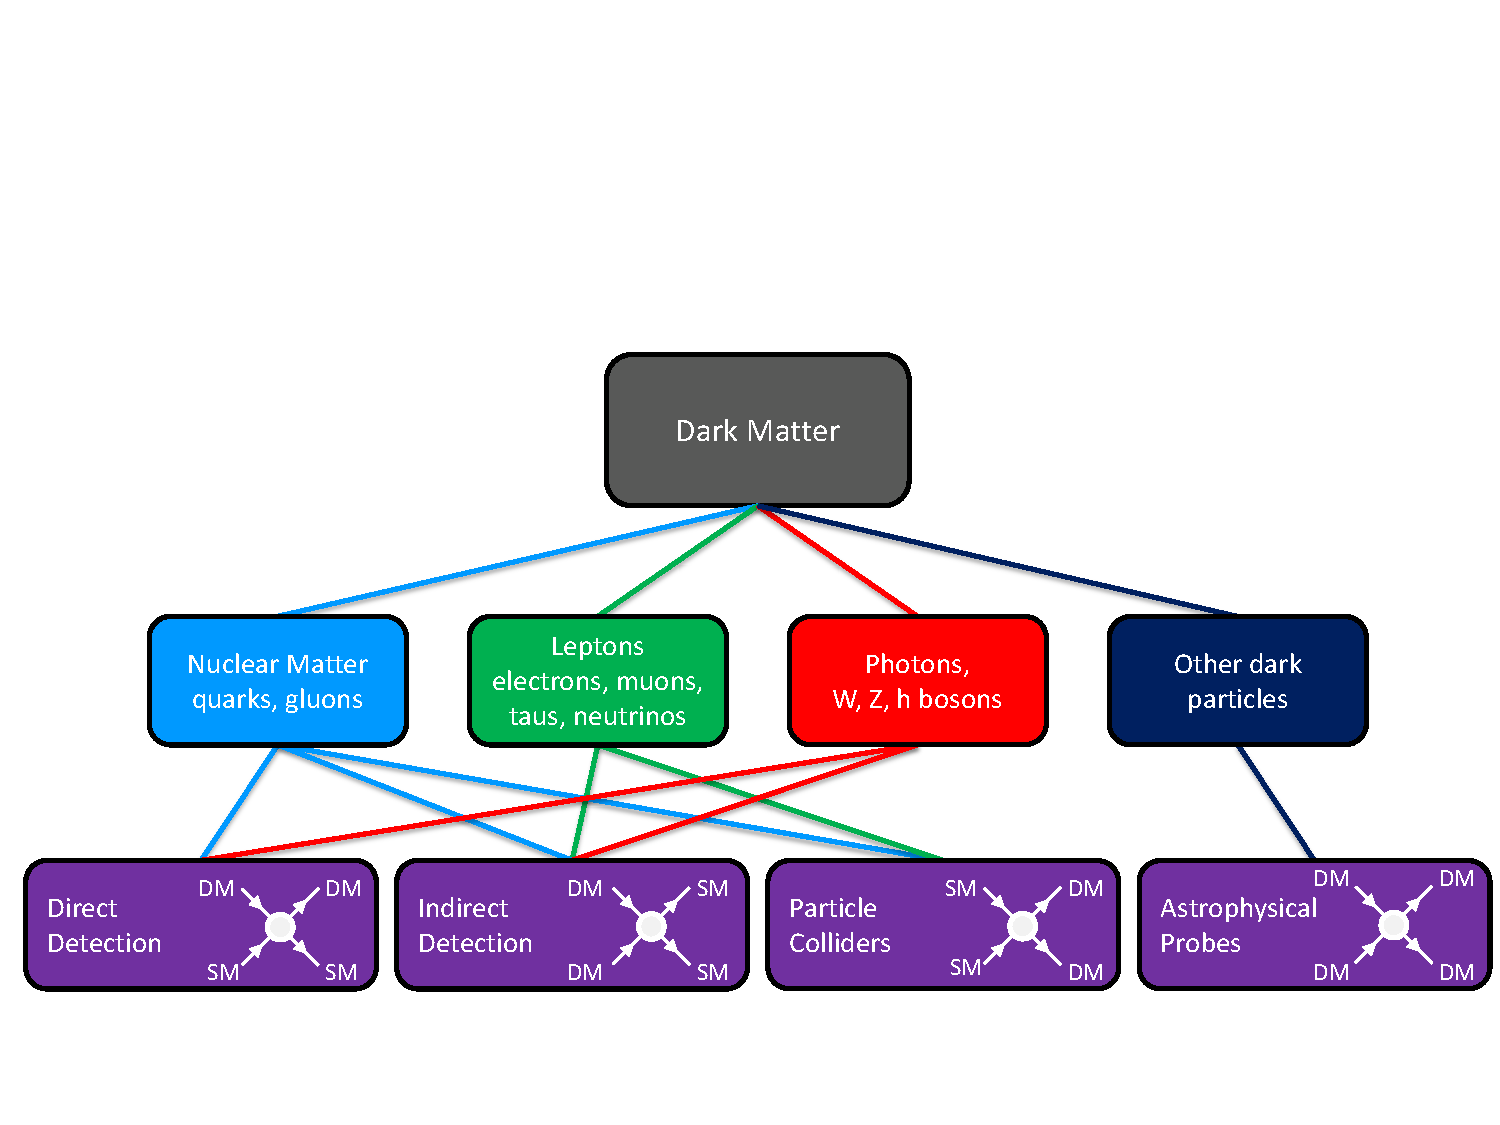
\includegraphics[width=0.85\textwidth]{figures/interactions.pdf}
\caption{
\label{fig:interactions}
Dark matter may have non-gravitational interactions that may be probed by four complementary approaches: 
direct detection, indirect detection, particle colliders, and astrophysical probes.
The lines connect the experimental approaches with the categories of particles that they most stringently probe (additional lines can be drawn in specific model scenarios). 
Figure taken from \citet{1305.1605} produced as part of Snowmass 2013.
\KB{Is it worth including a figure here to replace the ``conventional'' collider-direct-indirect dark matter search triangle? I'm thinking of something that people can easily re-use in talks and serves as a very simple visual to convey the importance of astrophysical probes.}
\ADW{I've added this figure, but I'm not sure it's exactly what we want (we talk about non-gravitational interactions . It'd be good to hear Annika and Matt B.'s input, since I think they've thought about this a lot.}
}
\end{figure}


\begin{deluxetable*}{l c c c}
\tabletypesize{\footnotesize}
\tablecaption{\label{tab:models} 
Probes of fundamental dark matter physics with LSST.}
\tablehead{
 \colhead{Model} & \colhead{Probe} & \colhead{Parameter} & \colhead{Value}
}
\startdata 
Warm Dark Matter (WDM) & Halo Mass & Particle Mass & \FIXME{$m_{\rm WDM} \sim 30 \keV$} \\
Self-Interacting Dark Matter (SIDM) & Halo Profile & Cross Section & \FIXME{$\sigma/m \sim 1 \cm^2/\g$} \\
Baryon-Scattering Dark Matter (BSDM) & Halo Mass & Cross Section & \FIXME{$\sigma \sim 10^{-26} \cm^2$} \\
Axion-Like Particles (ALPs) & Energy Loss & Coupling Strength & \FIXME{$g_{\phi e} \sim 10^{-13} \GeV^{-1}$} \\
Fuzzy Dark Matter (FDM) & Halo Mass & Particle Mass & \FIXME{$m \sim 10^{-21} \eV$}  \\
Primordial Black Holes (PBHs) & Compact Objects & Mass & \FIXME{$m \grsim \sim 10^{-12} \Msun$} \\
Weakly Interacting Massive Particles (WIMPs) & Indirect Detection & Cross Section & \FIXME{$\sigmav \sim 10^{-27} \cm^3/\second$} \\[+0.5em]
\enddata
\tablecomments{\ADW{There are clearly a lot of caveats on each line, but I think that a table like this would be very useful. I could use help here!}}
\end{deluxetable*}


